\lysh{34319}{4}

\begin{alist}
\item Το τριώνυμο $f(x) = 3x^2 + \kappa x - 4$ έχει διακρίνουσα:
$\Delta = \kappa^2 - 4 \cdot 3 \cdot (-4) = \kappa^2 + 48 > 0$, για κάθε $\kappa \in \mathbb{R}$
Άρα το τριώνυμο έχει για οποιαδήποτε τιμή του $\kappa$ δύο ρίζες πραγματικές και άνισες.

\item Για το γινόμενο των ριζών έχουμε:
\[P = x_1 x_2 = \dfrac{\gamma}{\alpha} = \dfrac{-4}{3} < 0.\]
Άρα, οι ρίζες είναι ετερόσημες.

\item Επειδή $x_1 < x_2$ και οι ρίζες είναι ετερόσημες, ισχύει ότι:
$x_1 < 0 < x_2$.
Επίσης είναι $\alpha < x_1$ και $x_2 < \beta$. Άρα:
$\alpha < 0$ και $0 < \beta$. (1)
Το πρόσημο του τριωνύμου φαίνεται στον παρακάτω πίνακα:

\begin{center}
\begin{tikzpicture}
\tikzset{t style/.style = {style = dashed}}
\tkzTabInit[color,lgt=3,espcl=2,colorC = maincolor!40,
colorL = maincolor!20,
colorV = maincolor!40]%
{$x$ / .8,$3x^2 +\kappa x - 4$ /0.8}%
{$-\infty$,$x_1$,$x_2$,$+\infty$}%
\tkzTabLine{ , $+$, z
, $-$ , z
, $+$ , }
\end{tikzpicture}
\end{center}

Από τον πίνακα προσήμου συμπεραίνουμε ότι:
$\alpha < x_1 \Rightarrow f(\alpha) > 0$ και $x_2 < \beta \Rightarrow f(\beta) > 0$ (2)
Από τις ανισώσεις (1) και (2) βρίσκουμε ότι $\alpha \cdot f(\alpha) < 0$ και $\beta \cdot f(\beta) > 0$, οπότε:
\[\alpha \cdot f(\alpha) \cdot \beta \cdot f(\beta) < 0.\]
\end{alist}
